\documentclass[12pt]{article}
\usepackage{amsmath}
\usepackage{graphicx}
\usepackage{listings}
\usepackage{longtable}
\usepackage{colortbl}
\usepackage{hyperref}
\usepackage{listings}
\usepackage{xcolor}
 

\lstdefinestyle{mystyle}{
    backgroundcolor=\color{white},  
    commentstyle=\color{olive},
    keywordstyle=\color{blue},
    numberstyle=\tiny\color{gray},
    numbers=left,
    numbersep=5pt,
    breaklines=true,
    postbreak=\mbox{\textcolor{red}{$\hookrightarrow$}\space},
    basicstyle=\ttfamily\small,
    frame=single,
    literate=*{+}{{\texttt{+}}}1,          % replace + with \texttt{+}
    keepspaces=true                        % keep original spacing
}
\lstset{style=mystyle}

 


\title{Floretions associated with A115032}
\author{Creighton Dement\thanks{floretionguru@gmail.com}}
\date{2023-10-07}

\begin{document}

\maketitle

\section{Purpose}
Since sequence  \href{https://oeis.org/A115032}{A115032} was submitted in 2006, several interesting formulae and results involving inscribed circles have been added by others (see links on OEIS page). This paper is only meant to show other sequences generated alongside this one (some not listed in the OEIS). Note this is not complete in any way- simply reordering A, B, and C, changing signs or adding "+ee" (binomial transform) or "-ee" (inverse binomial transform) will also produce related sequences. That is not a proof, just based on empirical evidence. 

\section{Floretions}

\subsection{Definition}

Every floretion has a representation as a tiling of an equilateral triangle. See \href{https://oeis.org/A308496}{A308496} for definition of 2nd-order floretions. The original definition of A115032 has 3 floretions A, B, and C and states the sequences is generated by "tes" of $A*B*C$ (\textit{tes} is just the real coefficient of the "ee" base vector)

 
\begin{figure}[h]
  \centering
  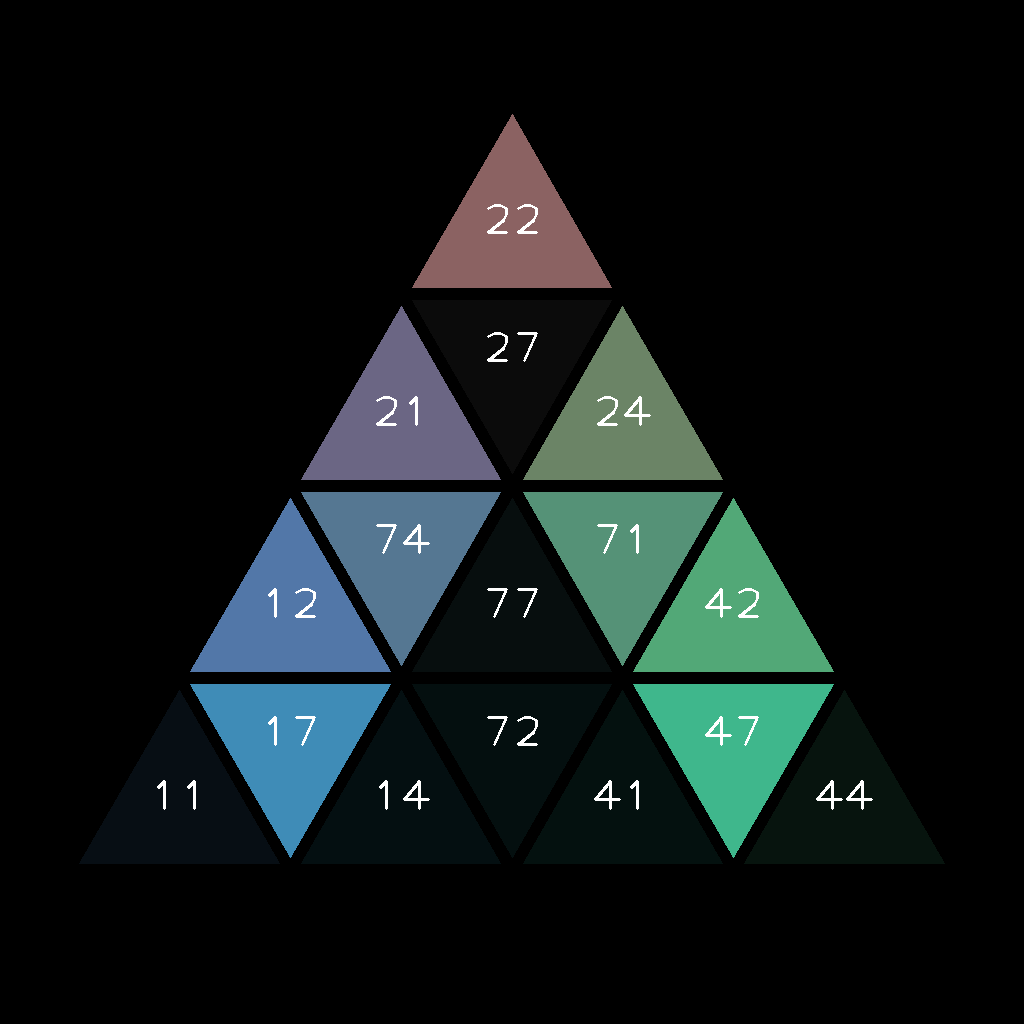
\includegraphics[scale=0.25]{order_2A115032_floA.png}
  \caption{Triangles (base vectors in octal) associated with $A = -ij + ie - ji - jj - jk - kj - ke + ei - ek$  } 
\end{figure}

\begin{figure}[h]
  \centering
  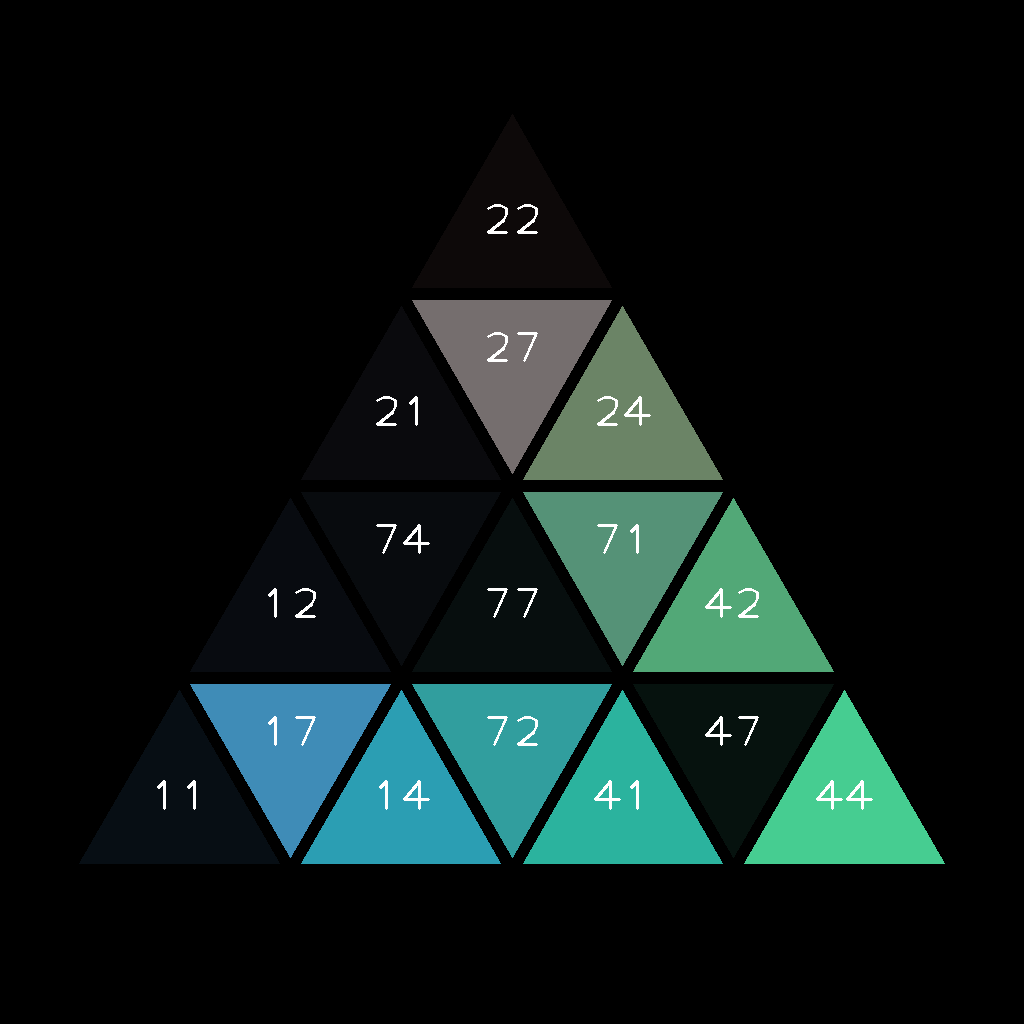
\includegraphics[scale=0.25]{order_2A115032_floB.png}
  \caption{Triangles (base vectors in octal) associated with  $B = -ik - ie - jk + je - ki - kj - kk - ei + ej$}
\end{figure}


\begin{figure}[h]
  \centering
  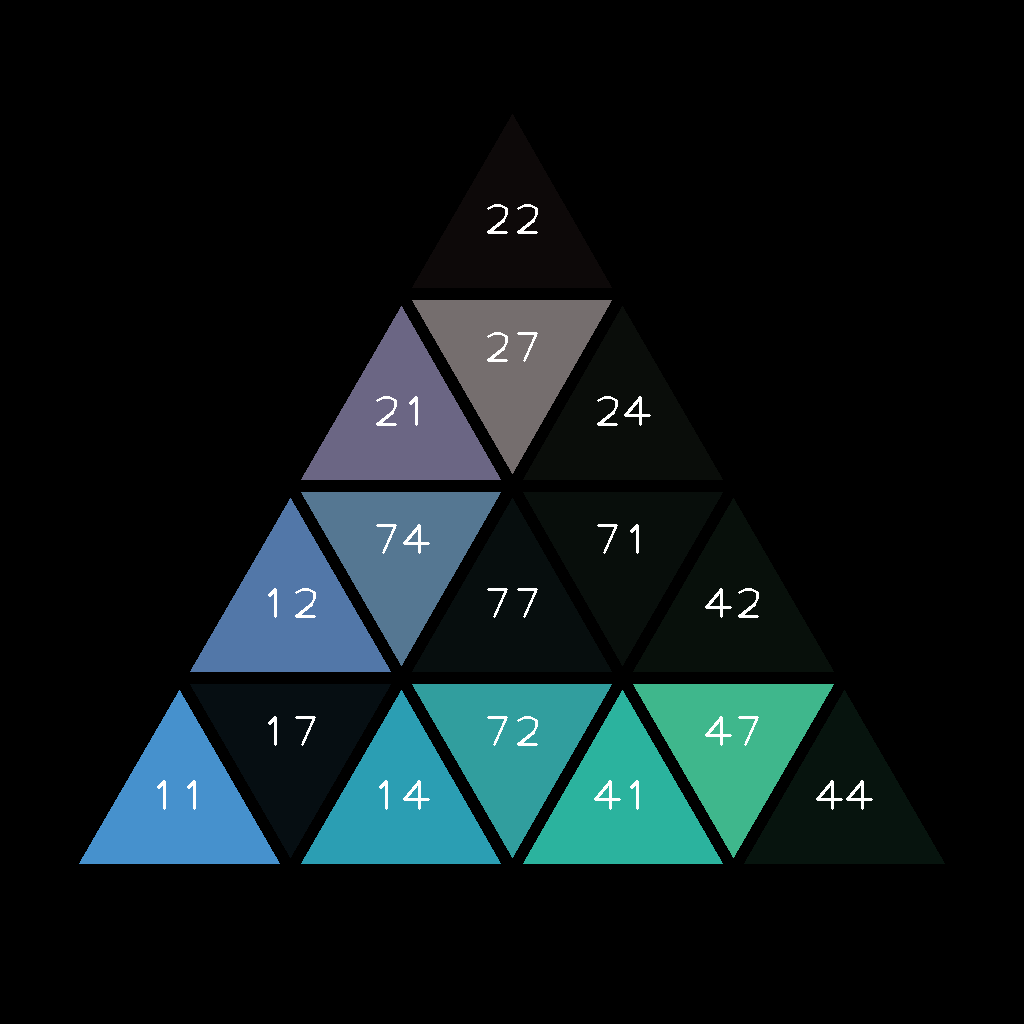
\includegraphics[scale=0.25]{order_2A115032_floC.png}
  \caption{Triangles (base vectors in octal) associated with  $C = -ii - ij - ik - ji - je - ki + ke - ej + ek$}
\end{figure}


\clearpage
 

\begin{align*}
  A*B*C &= +4.0\,ii - 4.0\,ij + 14.0\,ie - 4.0\,ji - 12.0\,jj \\
       &\quad - 8.0\,jk - 2.0\,je - 8.0\,kj + 12.0\,kk - 2.0\,ke \\
       &\quad + 14.0\,ei - 2.0\,ej - 2.0\,ek - 5.0\,ee, \\
  (A*B*C)^2 &= -64.0\,ii + 80.0\,ij + 8.0\,ik - 268.0\,ie + 80.0\,ji \\
           &\quad + 224.0\,jj + 152.0\,jk + 52.0\,je + 8.0\,ki + 152.0\,kj \\
           &\quad - 240.0\,kk + 36.0\,ke - 268.0\,ei + 52.0\,ej + 36.0\,ek \\
           &\quad + 81.0\,ee, \\
  (A*B*C)^3 &= +1140.0\,ii - 1444.0\,ij - 152.0\,ik + 4826.0\,ie \\
           &\quad - 1444.0\,ji - 4028.0\,jj - 2736.0\,jk - 950.0\,je \\
           &\quad - 152.0\,ki - 2736.0\,kj + 4332.0\,kk - 646.0\,ke \\
           &\quad + 4826.0\,ei - 950.0\,ej - 646.0\,ek - 1445.0\,ee.
\end{align*}

\subsection{Table}

\begin{longtable}{|c|c|c|c|c|}
    \( n \) & \( \text{ii} \) & \( \text{ij} \) \href{ https://oeis.org/A132584}{A132584} & \( \text{ik} \) \href{https://oeis.org/A053606}{A05360}    & \( \text{ie} \) \\
    \hline
    \( (A*B*C) \) & \( 4 \) & \( -4 \) & \( 0 \) & \( 14 \) \\
    \( (A*B*C)^2 \) & \( -64 \) & \( 80 \) & \( 8 \) & \( -268 \) \\
    \( (A*B*C)^3 \) & \( 1140 \) & \( -1444 \) & \( -152 \) & \( 4826 \) \\
    \( (A*B*C)^4 \) & \( -20448 \) & \( 25920 \) & \( 2736 \) & \( -86616 \) \\
    \( (A*B*C)^5 \) & \( 366916 \) & \( -465124 \) & \( -49104 \) & \( 1554278 \) \\
    \( (A*B*C)^6 \) & \( -6584032 \) & \( 8346320 \) & \( 881144 \) & \( -27890404 \) \\
    \( (A*B*C)^7 \) & \( 118145652 \) & \( -149768644 \) & \( -15811496 \) & \( 500473010 \) \\
    \( (A*B*C)^8 \) & \( -2120037696 \) & \( 2687489280 \) & \( 283725792 \) & \( -8980623792 \) \\
    \( (A*B*C)^9 \) & \( 38042532868 \) & \( -48225038404 \) & \( -5091252768 \) & \( 161150755262 \) \\
    \( (A*B*C)^{10} \) & \( -682645553920 \) & \( 865363202000 \) & \( 91358824040 \) & \( -2891732970940 \) \\

 \end{longtable}
\begin{longtable}{|c|c|c|c|c|}
    \( n \) & \( \text{ji} \) \href{ https://oeis.org/A132584}{A132584}& \( \text{jj} \) & \( \text{jk} \)\href{https://oeis.org/A053606}{ A05360} & \( \text{je} \) \\
    \hline
    \( (A*B*C) \) & \( -4 \) & \( -12 \) & \( -8 \) & \( -2 \) \\
    \( (A*B*C)^2 \) & \( 80 \) & \( 224 \) & \( 152 \) & \( 52 \) \\
    \( (A*B*C)^3 \) & \( -1444 \) & \( -4028 \) & \( -2736 \) & \( -950 \) \\
    \( (A*B*C)^4 \) & \( 25920 \) & \( 72288 \) & \( 49104 \) & \( 17064 \) \\
    \( (A*B*C)^5 \) & \( -465124 \) & \( -1297164 \) & \( -881144 \) & \( -306218 \) \\
    \( (A*B*C)^6 \) & \( 8346320 \) & \( 23276672 \) & \( 15811496 \) & \( 5494876 \) \\
    \( (A*B*C)^7 \) & \( -149768644 \) & \( -417682940 \) & \( -283725792 \) & \( -98601566 \) \\
    \( (A*B*C)^8 \) & \( 2687489280 \) & \( 7495016256 \) & \( 5091252768 \) & \( 1769333328 \) \\
    \( (A*B*C)^9 \) & \( -48225038404 \) & \( -134492609676 \) & \( -91358824040 \) & \( -31749398354 \) \\
    \( (A*B*C)^{10} \) & \( 865363202000 \) & \( 2413371957920 \) & \( 1639367579960 \) & \( 569719837060 \) \\
    \hline
  \end{longtable}


\begin{longtable}{|c|c|c|c|c|}
  \( n \) & \( \text{ki} \) \href{https://oeis.org/A053606}{ A05360}  & \( \text{kj} \) \href{https://oeis.org/A053606}{ A05360} & \( \text{kk} \) & \( \text{ke} \) \href{https://oeis.org/A207832}{ A207832} \\
  \hline
  \( (A*B*C) \) & \( 0 \) & \( -8 \) & \( 12 \) & \( -2 \) \\
  \( (A*B*C)^2 \) & \( 8 \) & \( 152 \) & \( -240 \) & \( 36 \) \\
  \( (A*B*C)^3 \) & \( -152 \) & \( -2736 \) & \( 4332 \) & \( -646 \) \\
  \( (A*B*C)^4 \) & \( 2736 \) & \( 49104 \) & \( -77760 \) & \( 11592 \) \\
  \( (A*B*C)^5 \) & \( -49104 \) & \( -881144 \) & \( 1395372 \) & \( -208010 \) \\
  \( (A*B*C)^6 \) & \( 881144 \) & \( 15811496 \) & \( -25038960 \) & \( 3732588 \) \\
  \( (A*B*C)^7 \) & \( -15811496 \) & \( -283725792 \) & \( 449305932 \) & \( -66978574 \) \\
  \( (A*B*C)^8 \) & \( 283725792 \) & \( 5091252768 \) & \( -8062467840 \) & \( 1201881744 \) \\
  \( (A*B*C)^9 \) & \( -5091252768 \) & \( -91358824040 \) & \( 144675115212 \) & \( -21566892818 \) \\
  \( (A*B*C)^{10} \) & \( 91358824040 \) & \( 1639367579960 \) & \( -2596089606000 \) & \( 387002188980 \) \\
  \hline
\end{longtable}

\begin{longtable}{|c|c|c|c|>{\columncolor{yellow}}c|}
  \( n \) & \( \text{ei} \) & \( \text{ej} \) & \( \text{ek} \) \href{https://oeis.org/A207832}{ A207832}  & \( \text{ee} \) \\
  \hline
  \( A*B*C \) & \( 14 \) & \( -2 \) & \( -2 \) & \( -5 \) \\
  \( (A*B*C)^2 \) & \( -268 \) & \( 52 \) & \( 36 \) & \( 81 \) \\
  \( (A*B*C)^3 \) & \( 4826 \) & \( -950 \) & \( -646 \) & \( -1445 \) \\
  \( (A*B*C)^4 \) & \( -86616 \) & \( 17064 \) & \( 11592 \) & \( 25921 \) \\
  \( (A*B*C)^5 \) & \( 1554278 \) & \( -306218 \) & \( -208010 \) & \( -465125 \) \\
  \( (A*B*C)^6 \) & \( -27890404 \) & \( 5494876 \) & \( 3732588 \) & \( 8346321 \) \\
  \( (A*B*C)^7 \) & \( 500473010 \) & \( -98601566 \) & \( -66978574 \) & \( -149768645 \) \\
  \( (A*B*C)^8 \) & \( -8980623792 \) & \( 1769333328 \) & \( 1201881744 \) & \( 2687489281 \) \\
  \( (A*B*C)^9 \) & \( 161150755262 \) & \( -31749398354 \) & \( -21566892818 \) & \( -48225038405 \) \\
  \( (A*B*C)^{10} \) & \( -2891732970940 \) & \( 569719837060 \) & \( 387002188980 \) & \( 865363202001 \) \\
  \hline
\end{longtable}

\begin{itemize}
  \item  \href{https://oeis.org/A207832}{ A207832: Numbers x such that $20*x^2$ + 1 is a perfect square} 
  \item \href{https://oeis.org/A053606}{ A05360: (Fibonacci(6*n+3) - 2)/4 }    
  \item \href{https://oeis.org/A132584}{A132584: a(n) = 18*a(n-1) - a(n-2) + 8 }   
 \end{itemize}
		 

\subsection{External Links}

\begin{itemize}
  \item GitHub repository: \url{https://github.com/Floretion-Inquisitor/floretions}
  \item Code example for A115032: \url{https://github.com/Floretion-Inquisitor/floretions/tree/main/examples/A115032}
  \item Wiki: \url{https://github.com/Floretion-Inquisitor/floretions/wiki}
  \item Explanation of 2nd order floretions at the OEIS: \url{http://www.mrob.com/pub/seq/floretion.html}

\end{itemize}

 


\end{document}